%\chapter*{Introduction}\addcontentsline{toc}{chapter}{Introduction}
\section{Introduction}

Seaborne monitoring and measurements are often expensive and time consuming, though they can have a large impact on the area, where the data have been obtained. In 2011 the naval safe zone around the Fukusima accident was laid down based only on estimates of the radiation contamination\cite{fukushima}, because low amount of measurement data was available due to high measurement costs and risks. Another notable area in need of thorough oceanographic surveying is the area of Greenland, because its coastal waters are very poorly mapped up to present day\cite{2009AGUFMOS21A1152W}. Ships have to sail in a roundabout way around the island, because the risk of wrecking in unknown littoral area is very high. This is a huge waste of time and natural resources annually, but complete bathymetric survey of the danger zone is impossible due to the shortages of funds and manpower.

\subsection*{Oceanography and Bathymetry}

Not many people come across these expressions often. Oceanography can be summarized as a branch of Earth science that studies the ocean. It includes a wide range of topics, like the study of marine ecosystem, ocean currents, plate tectonics and the geology of the sea floor. Bathymetry is the study of underwater depth of lake or ocean floors. The advancing technology allows even more possibilities, like the aforementioned radiological measurements, or general monitoring of the seas. These areas are not the only possible applications, but they are relatively straightforward and general for easy demonstration.

\subsection*{Advantages of autonomous vessels}

Oceanographic measurements today are carried out by large crewed ships, but in many cases they could be replaced by a number of smaller crafts, in order to reduce time and cost and increase the available manpower in other tasks. These vessels have the ability to sail previously unsurveyable areas as well, thanks to the shallower draught and smaller size. Although the number of Autonomous Underwater Vehicles (AUV) are rapidly increasing\cite{AUV_growth}, the the Unmanned Surface Vehicles (USV) are still used mostly for military and academic purposes\cite{USV_applications}.

[Fleet class USV wrapfigure]

\subsection*{Limitations}

The most notable limitation of the current mobile robotic technologies are their small size itself. This results in relatively small range based on their smaller power capabilities, and narrow field of application. Conventional electric powered boats can operate reliably only in the littoral or riverine zones, where the mission area is relatively small.

\subsection*{Scope of duties}

The goal of this project is to develop an autonomous surface vehicle, which is capable of conducting multiple seaborne measurements. In order to execute an oceanography mission, the ship must be capable of autonomous navigation based on Global Positioning System (GPS) and an Internal Measurement Unit (IMU), to further enhance the precision in hazardous environment.

\begin{figure}[H]
	\centering
	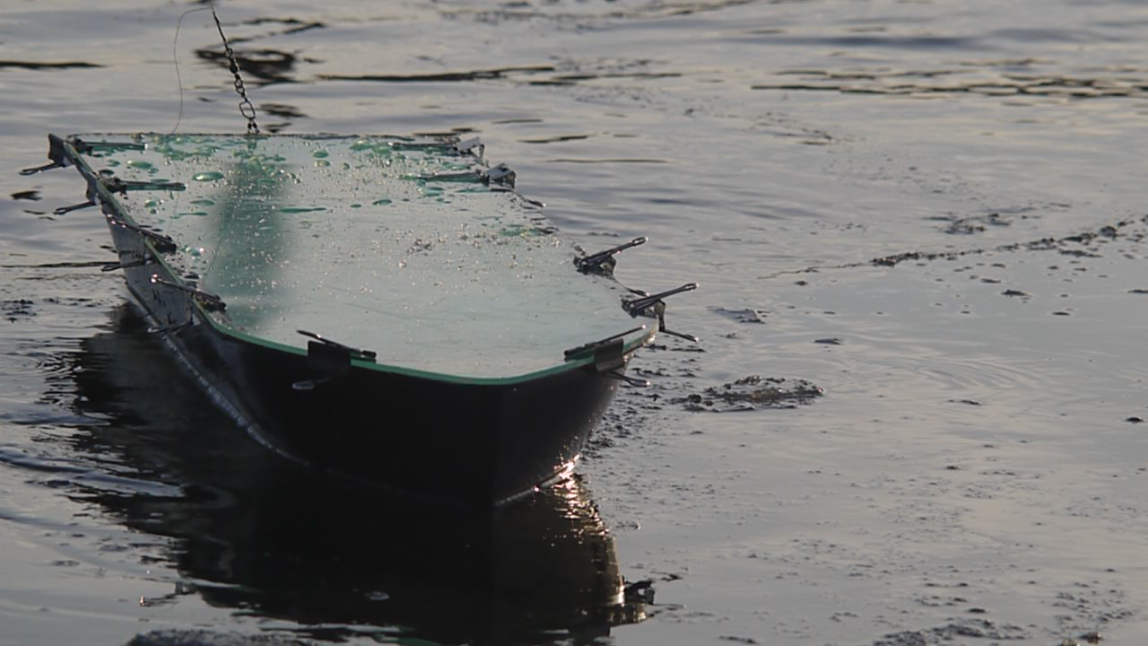
\includegraphics[width=0.8\textwidth]{img/aauship}
	\caption{The AAUSHIP prototype on her maiden voyage}
	\label{fig:aauship}
\end{figure}

\subsection*{Development guidelines}
To keep a sensible and extendable system, the control software of the ship follows the guidelines of the Model-Based Design approach. The system software can be divided to two different modules, one that is dependent, and one that is independent from the physical characteristics of the vessel. In order to maximize the extendability of the system, the fix (independent) modules must be completely general, but as thorough as possible, in order to keep the complexity of the changeable (dependent) software of the robot minimal.
\begin{wrapfigure}{r}{0.48\textwidth}
  \begin{center}
    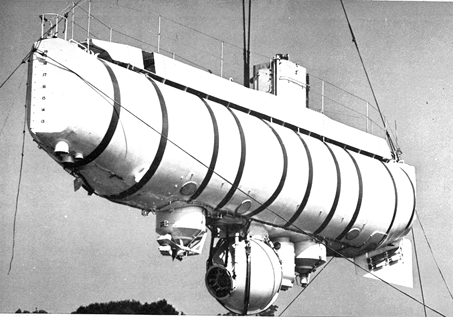
\includegraphics[width=0.5\textwidth]{img/trieste}
  \end{center}
  \caption{Bathyscaphe Trieste, the first manned vessel that reached the bottom of Challenger Deep (Mariana Trench)\cite{trieste}}
\end{wrapfigure}
